%# -*- coding: utf-8-unix -*-
%%==================================================
%% chapter02.tex for SJTU Master Thesis
%% related work
%%==================================================
%\bibliographystyle{sjtu2}%[此处用于每章都生产参考文献]

\chapter{ 相关工作 }
\label{chap:related}

\section{相似度方程定义}
\label{sec:similarityfunc}
相似轨迹查询工作在某种意思上和时序数据相似查询共享一些方法定义。相似轨迹查询的首要步骤通过某种选定轨迹与轨迹点间的距离度量来定义相似度(或称为距离)方程,之后是设计高效的查询过程算法来解决从大规模数据库中找到符合要求的备选轨迹。定义相似度方法在过去有许多深度的讨论,之前的工作有通过利用离散傅里叶变化(Discrete Fourier Transform)[Ref bylocation2]将轨迹数据转化为多维空间上的点,任何通过比较这些点在特征空间上的欧式距离来比较轨迹数据时间的相似性。之后有科研人员在此工作成果的基础上通过改善实现子轨迹的匹配查询,并验证了离散小波变换(Discrete Wavelet Transform)的可行性。切比雪夫多项式(Chebyshev polynomials)在轨迹近似和索引方面有被证明是可应用的。但是这些方法的前提调前是需要轨迹上时序上具有相同的长度,因此这些转变返程所提供的相似度方法不适用与本文所提出的相似轨迹查询。
\\

\begin{figure}[!htp]
  \centering
  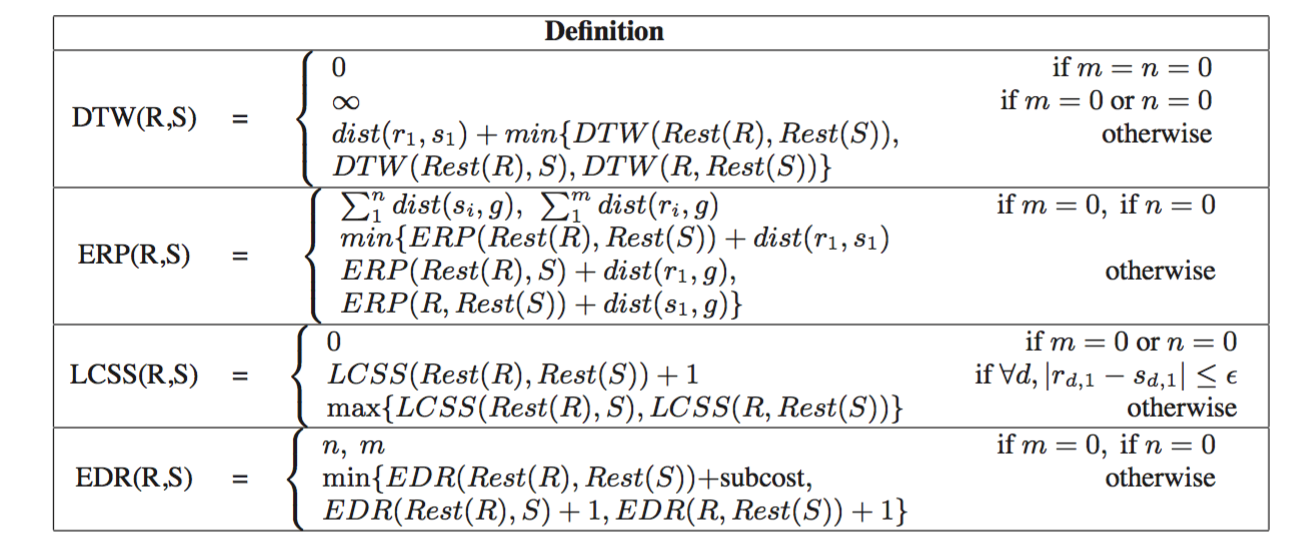
\includegraphics[width=1.0\textwidth]{chapter02/definition.png}
  \bicaption[fig:2-1]{这里将出现在插图索引中}{相似度函数定义\footnotemark[1]}{Fig}{Definition of distance functions}
\end{figure}
\footnotetext[1]{$dist(ri,si)=$ L1 or L2 norm; $subcost = 0$ if $r1,t−s1,t$, else $subcost= 1$}

图\ref{fig:2-1}是典型且常用的相似度方程定义。这些方程根据自身特点与优势应用于不同的场景中,包括欧氏距离方程(Euclidean Distance),动态时间规整(Dynamic Time Warping),最长公共子序列算法(Longest Common Subsequence),基于编辑代价的方法(Edit Distance With Real Penalty)和基于序列编辑的距离方法 (Edit Distance on Real Sequences)。动态时间规整(DTW)方法在比较轨迹之间相似性的过程中采用了时间偏移(time-shifting)来使得轨迹中的一些点可以尽可能多地重复出现以实现最好效果的校准。但这种方法在原有轨迹数据点出现误差(或称为噪声点)的时候会影响比较的准确性因为所有的点都需要被匹配。相比如动态时间规整方法(DTW),最长公共子序列(LCSS)选择忽略某些点以避免对他们的重排序过程,从结果上而言这种方法舍弃了偏离采样的误差点以提高了准确性,但需要人为预定距离阈值以判断什么数据属于误差点。基于编辑代价的距离方法(EDR)与LCSS方法类似,他们最初提出是为了解决字符串匹配问题,在轨迹数据匹配这一方面他们均采用一个阈值参数来判断两个点是否匹配,但EDR考虑了距离之间的衡量代价以决定是否将两个点进行匹配。在此基础上基于序列编辑的距离方法(ERP)结合EDR和DTW方法选择固定点进行距离计算。

相似度方法通常根据具体的应用进行具体的选取。但上述的相似度方法主要是基于轨迹与轨迹之前相似度的查询,在本文设计的相似轨迹查询方法上的应用度并不理想,本工作的查询条件是基于一组地理坐标点的查询,并且工作更关注与一条轨迹是否能够很好地连接上给定的一组查询点,从而提供基于轨迹点的相似轨迹结果。因此,在这样的情景下,我们需要定义一个新的相似度方程。
\\

\section{轨迹数据预处理}
\label{sec:preprocess}

\subsection{WGS84坐标系统转换至GCJ-02坐标系统}
\label{subsec:coord-transform}
WGS84(World Geodetic System1984)坐标系统是GPS数据所基于的坐标系统,这一坐标系是通过世界卫星观测站所检测到的地理坐标。这一坐标系并不能直接应用在中国国家的地图坐标显示中,因为中国国家会测局在地理信息系统中使用的是基于GCJ-02的坐标系统,这一坐标系统也称为火星坐标系统。如果直接将WGS84坐标数据应用于使用GCJ-02的地图显示接口,则会造成100米到700米范围内的显示误差。同理,用户使用GCJ-02地图点击获得的地理位置查询点也会在相似轨迹查询中因为与WGS84坐标系统的偏差因素造成查询结果的不准确性。在轨迹预处理最开始先将WGS84坐标数据根据已有的算法\footnotemark[1]参考转换成GCJ-02系统下的坐标
\footnotetext[1]{https://github.com/googollee/eviltransform}
\\


\subsection{轨迹数据简化}
\label{subsec:trajectory simplification}
轨迹数据预处理中,轨迹数据的简化(或压缩)是比较重要一步。轨迹数据简化主要是指在保证轨迹的可利用性与大致准确的同时减少轨迹的点数目,以达到轨迹数据的传输、处理和存储上减少开销的目的。在本文的应用场景中,我们首先采用\emph{Douglas}–\emph{Peucker}算法来完成我们的轨迹简化任务。该算法的主要思路在于将通过分而治之,将曲线轨迹表示成一系列点的方法,从而减少点的数目。如今GPS的数据采样通常较为频繁,因此在我们对轨迹处理的范围上来所,我们可以近似地将我们所运用的数据集中的轨迹看成是一条连续的曲线,通过\emph{Douglas}–\emph{Peucker}算法以及我们人为设定简化阈值,我们可以高效且合理地进行轨迹简化。

\begin{algorithm}
% \begin{algorithm}[H] % 强制定位
\caption{Douglas-Peucker算法}
\label{algo:dp-ts}
\begin{algorithmic}[1] %每行显示行号
\Require 一条原始轨迹数据$Traj$, 简化阈值$\epsilon$ % 输入
\Ensure 简化后的轨迹$Traj'$ % 输出
\State $dis\_max \gets 0$;$index \gets 0$
\For{$i = 1$ to $Traj.length-1$}
	\State $temp\_dis \gets$ Traj[i]'s perpendicular Distance to Line(Traj[0], Traj[Traj.length])
	\If{$temp\_dis > dis\_max$}
		\State $dis\_max \gets temp\_dis$;$index \gets i$
	\EndIf
\EndFor
\If{$dis\_max > \epsilon$}
	\State half\_left $\gets Douglas$-$Peucker(Traj[0:index],\epsilon)$;
	\State half\_right $\gets Douglas$-$Peucker(Traj[index:Traj.length],\epsilon)$;
	\State $res \gets$ half\_left $\bigcup$ half\_right;
	\Else
	\State $res \gets \{Traj[0], Traj[Traj.length]\}$;
\EndIf	
\State \textbf{return} $res$;
\end{algorithmic}
\end{algorithm}

算法\ref{algo:dp-ts}在首先连接轨迹首尾两点$Traj[0],Traj[Traj.length]$,遍历轨迹一遍得到离线段距离最大的点$Traj[index]$,计算该距离并与预先设定的阈值$\epsilon$比较。如果大于阈值$\epsilon$,则将轨迹以$Traj[index]$为中点分为两端,迭代重复上述工作;如果小于阈值$\epsilon$,则直接将线段段作为曲线的近似以做简化。当曲线完成上述任务,依次连接处理好的子线段,完成轨迹简化任务。
\\

\section{轨迹数据索引与获取}
\label{sec:index}
空间数据结构对从一个大规模轨迹数据集中获取特定轨迹数据是十分重要的。效率问题是查询大规模数据库或数据集来获取信息的首要考虑因素。而查询效率十分依赖于合理的轨迹索引。轨迹数据根据数据特点的不同姓对索引技术也有着特殊的要求。目前主流的索引技术主要有三类:1)基于空间维度的索引,利用R树(R-tree)索引进行查询。通过3DR树(3D R-tree)或者STR树(STR-tree)进行带有时间维度的查询;2)利用多版本的数据结构,根据特定情况使用 MR树(MR-tree)、HR树(HR-tree)、MV3R树(MV3R-tree)等等;3)将空间划分网格结构然后对应每个网格建立对应的空间索引,这类数据结构包括MTSB树(MTSB-tree)和SETI。本文中我们使用R树这一最基本的数据结构,其满足我们对算法的实现需求。

R树数据结构在空间数据库中应用广泛,许多轨迹索引结构大体上是基于R树进行拓展。R树结构是一个平衡树结构,R树中的每一个节点代表包含其所有子节点一个区域,这个区域通常被称为最小区域箱(Minimum Bounding Box)。节点中的每一个数据体指向对应的子节点的最小区域箱信息。R树搜索的关键字是最小区域箱中的每一个节点。如图\ref{fig:2-2}所示的是R树数据结构的2种表现形式。在\ref{fig:2-2}(b)中我们看到树结构而图\ref{fig:2-2}(a)描述了数据和最小边界箱是如何分布在空间中的。
\\

\begin{figure}[!htp]
  \centering
  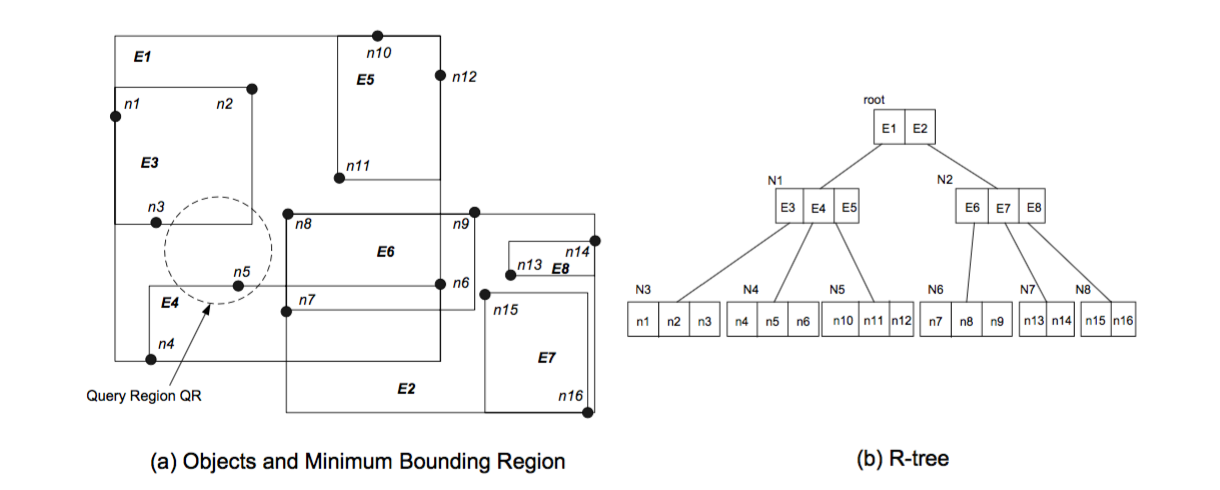
\includegraphics[width=1.0\textwidth]{chapter02/rtree.png}
  \bicaption[fig:2-2]{这里将出现在插图索引中}{R树数据结构举例}{Fig}{Two views of an R-tree example}
\end{figure}

在图\ref{fig:2-2}中,根节点有两个数据体$E1$,$E2$,分别对应子节点$N1$,$N2$。$N1$代表的最小边界箱包含了其子节点$N3$、$N4$、$N5$以及数据体$E1$所具有的最小边界箱信息。值得注意的是空间点的体现只有在R树的叶节点上。R树可以应用在范围查询和近邻查询中。本文主要使用R树近邻查询这一属性。给定一个查询点,R树可以通过最优优先搜索(best-first)和深度优先搜索(depth-first)两种树遍历策略找到在数据集中最接近查询点的数据。在两种搜索策略中,查询点和每一个最小边界箱的距离被定义为变量$mindist$。之后的搜索过程基本遵从两种搜索策略各自算法。

在R树中插入一个新的节点大致需要以下几个步骤。当有新的轨迹数据需要被添加到已有的R树种,首先为待插入的轨迹数据点找到一个合适插入的子节点中。再寻找叶结点的过程中我们会选择符合最小边界范围且对R树扩展度最小的一个叶结点。然后若找到R树叶结点数据溢出,那么我们需要对叶子结点进行分裂操作;若没有溢出,则可以将待添加的轨迹数据加入到当前已经找到的叶子节点中。最后对R树进行变换向上传递并对树高进行增高以完成插入操作。删除操作近似于插入过程的逆过程,在此不予以赘述。
\\

%\section{k最近邻算法}
%\label{sec:knn}

\section{本章小结}
\label{sec:conclusion2}
本章节中,本文通过图标和伪代码讨论了相似轨迹查询方法的设计与实现的基本相关工作,对本文所应用的基本定义、处理思路和数据结构有了一个初步的了解。根据本文场景定义个性化的相似度方程后,我们在查询阶段需要通过多点输入的条件下进行归集查询。由于输入数据的轨迹点数目相对较少,我们可以借助已有的数据结构进行空间距离上搜索。利用R树和基于k最邻近的进行方法拓展是本文实现算法的基本思想,以快速的搜索并获取数据。根据上述本文工作相关工作描述,我们可以得出实现本文算法的先决条件目前都是基于只有已有的成熟工作。在下一章节中,本文将开始对相似轨迹查询方法进行理论讨论。